\datos{color}{}{}
\section*{Tarea 1: experimento de control de posición de un robot móvil.}
\addcontentsline{toc}{section}{Tarea 1: experimento de control de posición de un robot móvil.}

El experimento consiste en controlar la posición de un robot móvil con el
Simulador CoppeliaSim. Los pasos a llevar a cabo son los siguientes:

\subsection*{1. Descargar el simulador y agregar el modelo del robot al mismo como se
explica en el documento Interfaz de la Práctica.}
\addcontentsline{toc}{subsection}{1. Descargar el simulador y agregar el modelo del robot al mismo como se
explica en el documento Interfaz de la Práctica.}

Se ha creado una imagen de \textit{Docker} con el simulador instalado, el modelo del robot
\textit{Khepera IV}, y el \textit{framework ROS2}. En el apartado \ref{} se detalla la descarga 
e instalación utilizando \textit{Docker}. En la Figura \ref{fig:t1.2} se observa que el robot se 
ha cargado correctamente.

\subsection*{2. Al arrastrar el robot desde el panel lateral y soltarlo en el espacio de
trabajo, el robot quedará agregado a la simulación.}
\addcontentsline{toc}{subsection}{2. Al arrastrar el robot desde el panel lateral y soltarlo en el espacio de
trabajo, el robot quedará agregado a la simulación.}

En la Figura \ref{fig:t1.2} se observa que el robot se 
ha agregado correctamente a la simulación.

\begin{figure}[H]
    \begin{center}
    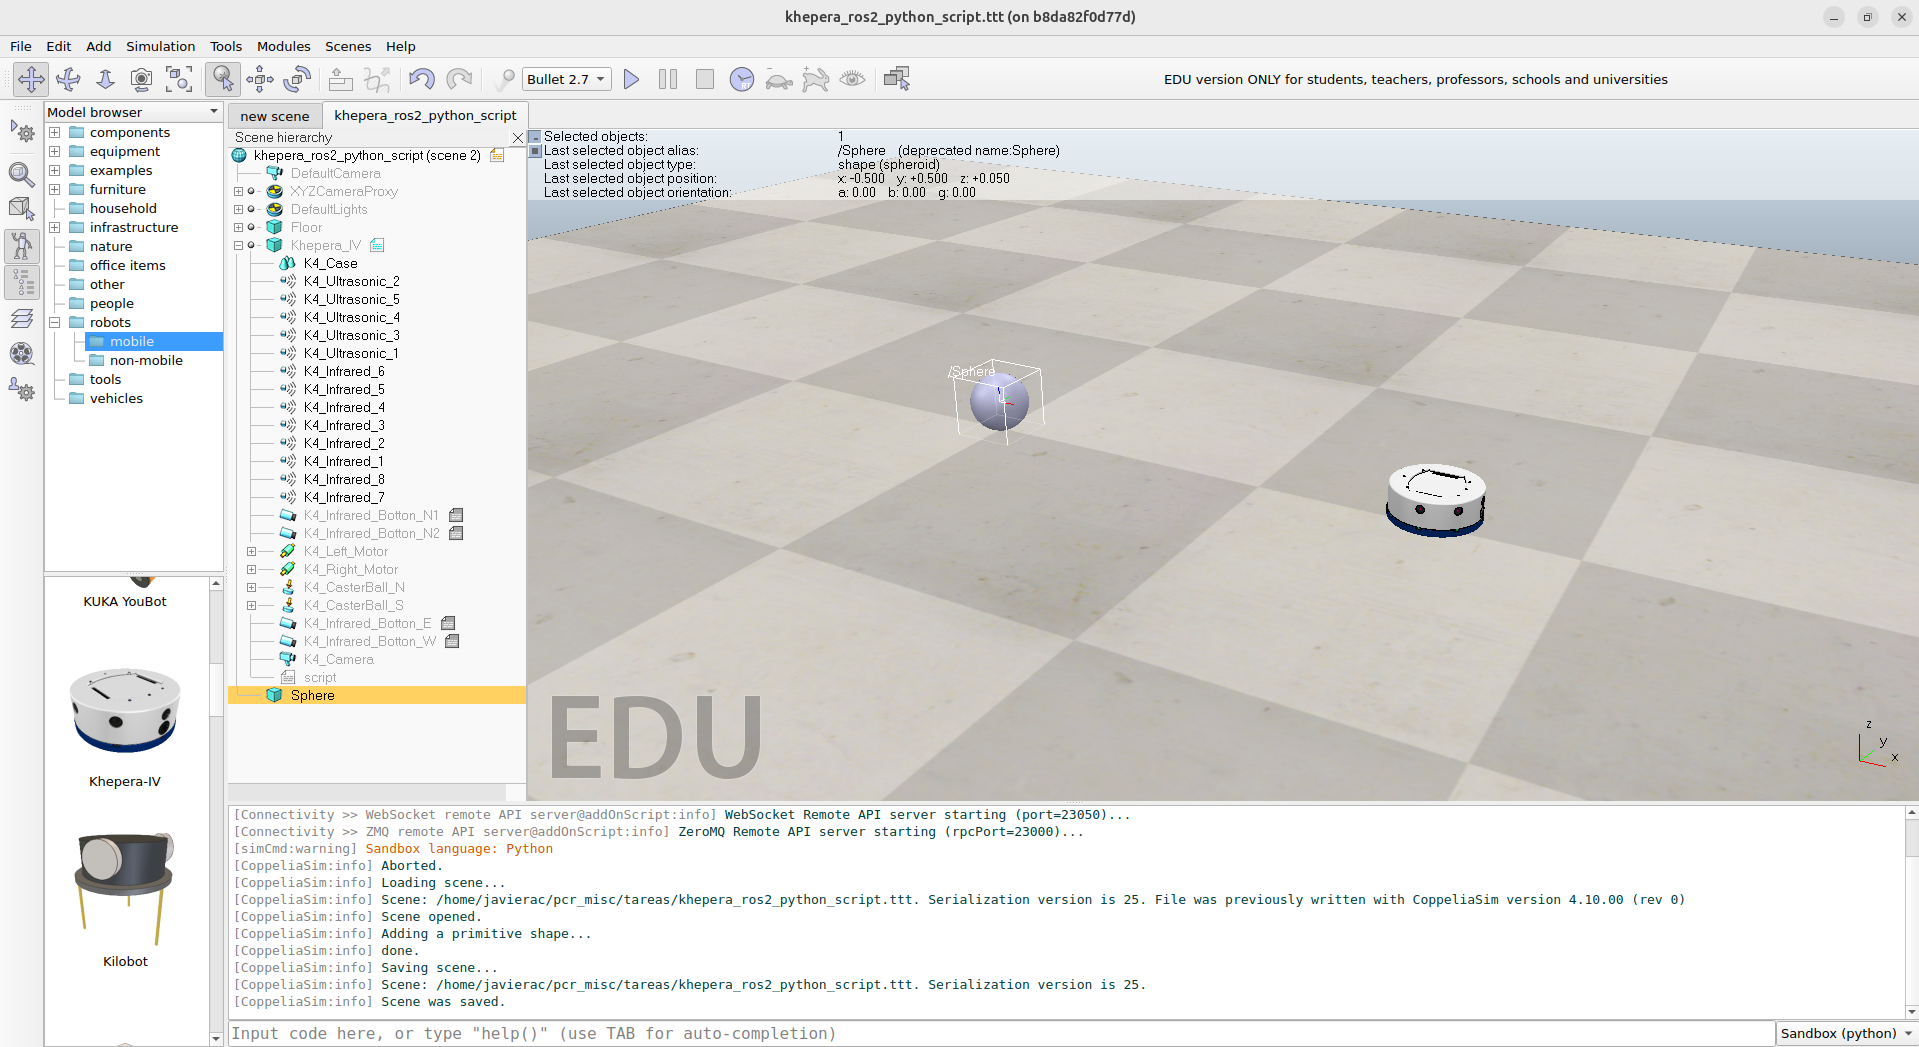
\includegraphics[scale=0.2, angle=0]{Images/tarea1/robot.png}
    \caption{\label{fig:t1.2} Robot \textit{Khepera IV} y objeto que representa el
    punto de destino agregados a \textit{Coppelia Sim}.}
    \end{center}
\end{figure}

\subsection*{3. Iniciar la simulación y observar el comportamiento del robot. ¿A qué se
debe este comportamiento?}
\addcontentsline{toc}{subsection}{3. Iniciar la simulación y observar el comportamiento del robot. ¿A qué se
debe este comportamiento?}

\subsection*{4. Abrir el script de programación del robot y observar los valores de las
velocidades izquierda y derecha.}
\addcontentsline{toc}{subsection}{4. Abrir el script de programación del robot y observar los valores de las
velocidades izquierda y derecha.}

El robot se mueve dibujando una trayectoria en arco de circunferencia, Figura \ref{fig:t1.3_2}. Haciendo doble click en el script por defecto del robot,
Figura \ref{fig:t1.3}, se abre el script que se presenta en el Código \ref{cod:t1.3}. Este comportamiento
se debe a las velocidades angulares ($w_L,\; w_R$) asignadas a cada motor: 3 rad/s al izquierdo y 5 rad/s al derecho,
respectivamente. Por tanto, el motor izquierdo gira más lento que el derecho y el robot realiza una trayectoria
en arco de circunferencia de radio $R = 0.176 \text{ metros}$, que se obtiene mediante la Ecuación (1) conociendo
la distancia entre los centros de las ruedas (\textit{axle track}), $L = 0.088 \text{ metros}$.

\begin{equation}
R = \frac{L}{2} \cdot \frac{\omega_R + \omega_L}{\omega_R - \omega_L}
\end{equation}

\begin{figure}[H]
    \centering

    \begin{minipage}{0.48\textwidth}
        \centering
        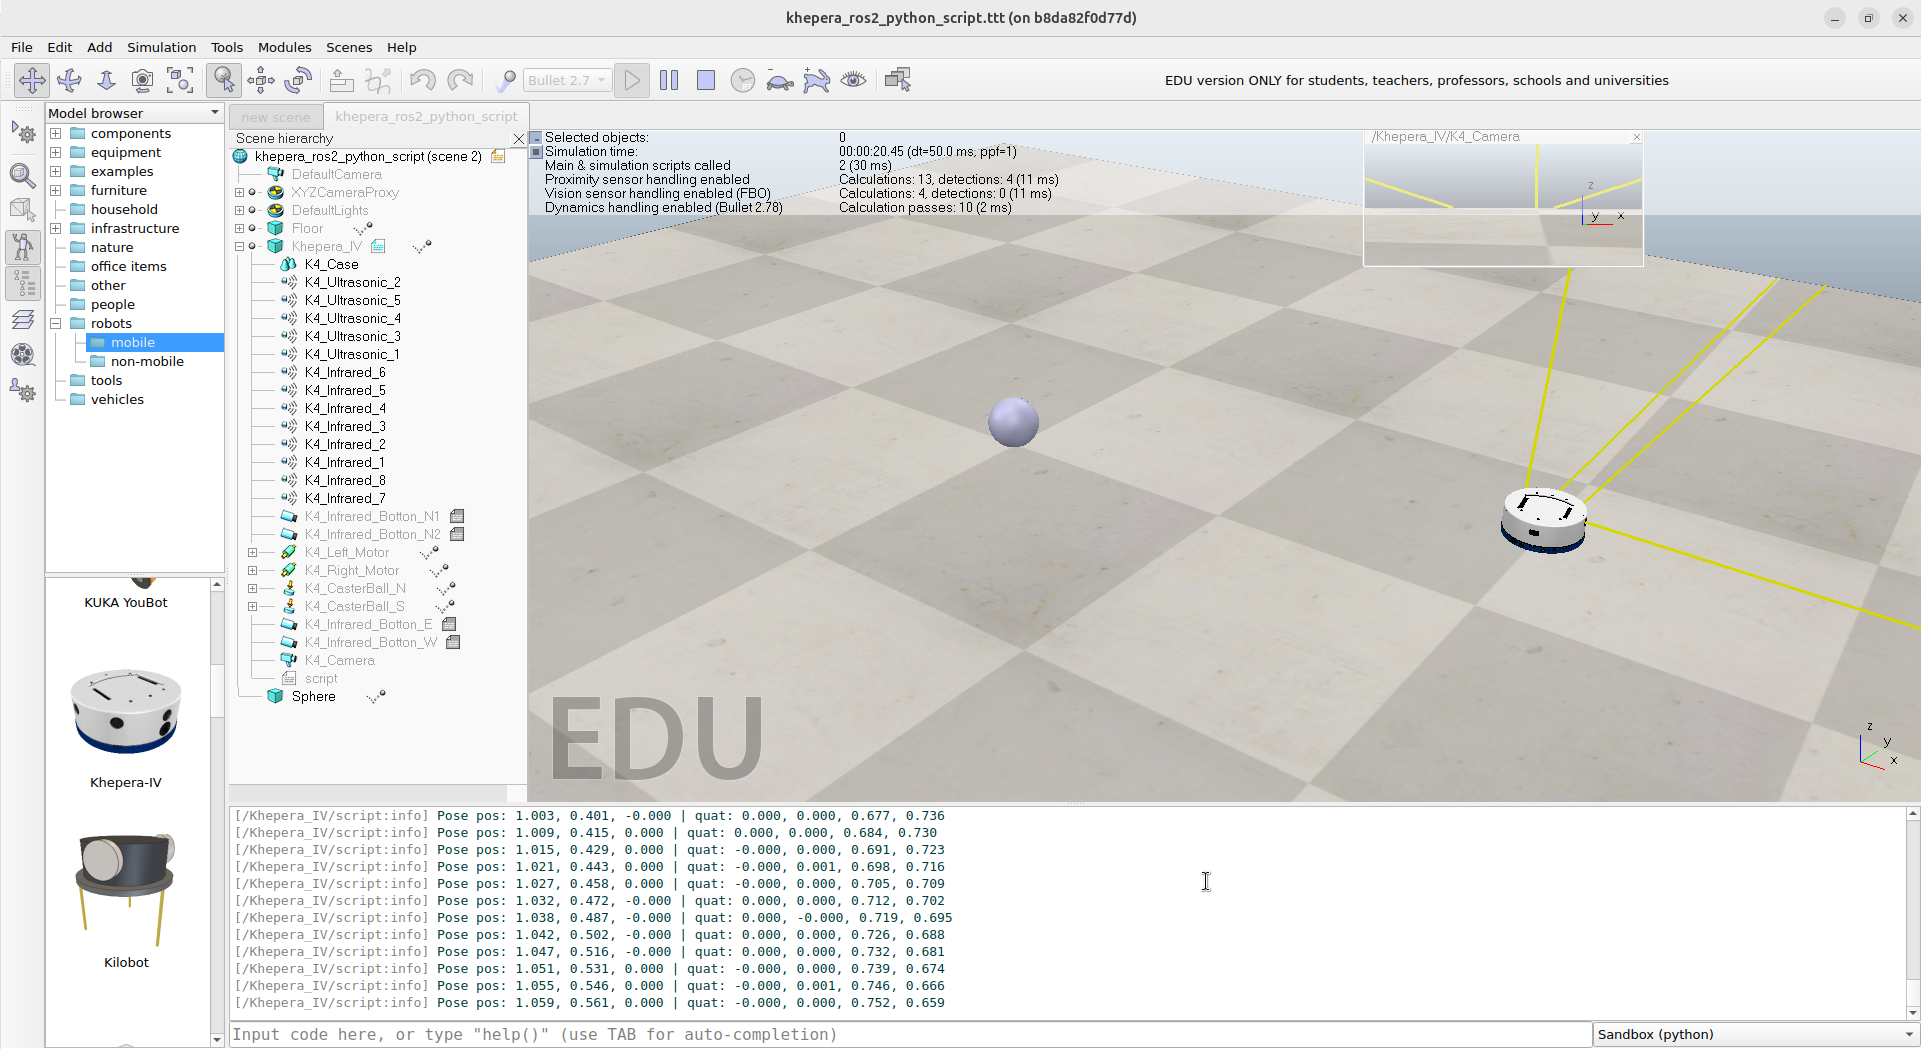
\includegraphics[scale=0.16]{Images/tarea1/trayectoria_por_defecto.png}
        \caption{\label{fig:t1.3_2} Trayectoria por defecto.}
    \end{minipage}
    \hfill
    \begin{minipage}{0.35\textwidth}
        \centering
        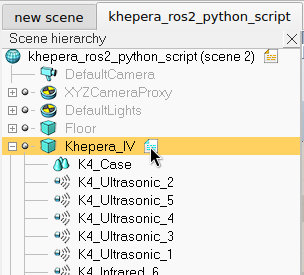
\includegraphics[scale=0.5]{Images/tarea1/script.png}
        \caption{\label{fig:t1.3} Script por defecto del robot.}
    \end{minipage}

\end{figure}

\begin{comment}
    \begin{figure}[H]
    \begin{center}
    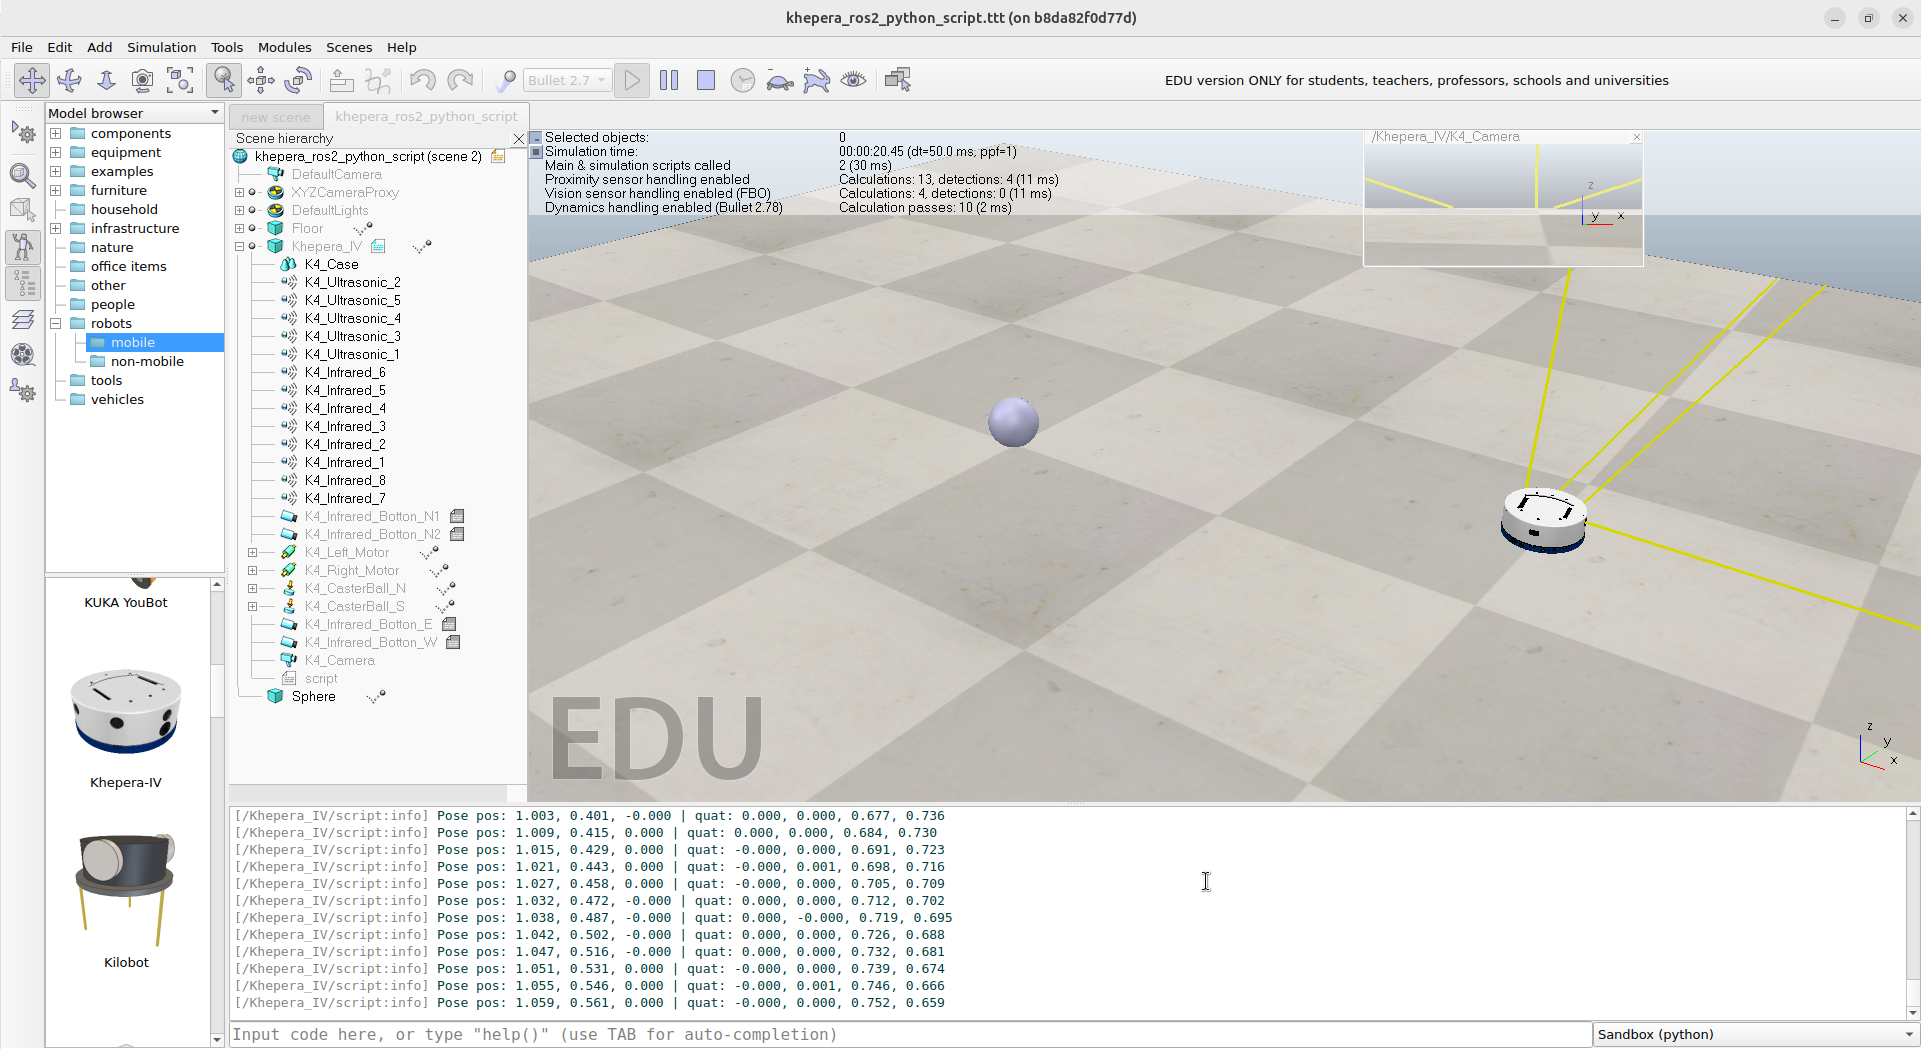
\includegraphics[scale=0.5, angle=0]{Images/tarea1/trayectoria_por_defecto.png}
    \caption{\label{fig:t1.3_2} Trayectoria por defecto.}
    \end{center}
\end{figure}

\begin{figure}[H]
    \begin{center}
    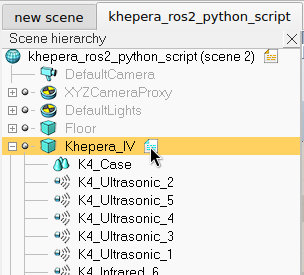
\includegraphics[scale=0.5, angle=0]{Images/tarea1/script.png}
    \caption{\label{fig:t1.3} Script por defecto del robot.}
    \end{center}
\end{figure}
\end{comment}

\lstinputlisting[style=luastyle, caption={Script por defecto del robot.}, label={cod:t1.3}]{Code/tarea1/script_por_defecto.lua}


\subsection*{5. Agregar a la simulación un objeto que represente el punto de destino del
robot.}
\addcontentsline{toc}{subsection}{5. Agregar a la simulación un objeto que represente el punto de destino del
robot.}

Se ha añadido una esfera con las propiedades descritas en la Figura \ref{fig:t1.5} y en la posición
$(x,\; y,\; z) = (-0.5,\; 0.5,\; 0.05)$, como se observa en la Figura \ref{fig:t1.2}.

\begin{figure}[H]
    \begin{center}
    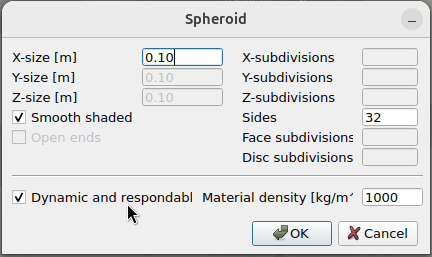
\includegraphics[scale=0.5, angle=0]{Images/tarea1/esfera.png}
    \caption{\label{fig:t1.5} Propiedades de la esfera añadida como punto de destino.}
    \end{center}
\end{figure}


\subsection*{6. Con las coordenadas del punto de destino y las del robot, calcular las
velocidades angular y lineal para controlar su posición.}
\addcontentsline{toc}{subsection}{6. Con las coordenadas del punto de destino y las del robot, calcular las
velocidades angular y lineal para controlar su posición.}

\subsection*{7. Obtener las velocidades que se envían al robot (izquierda y derecha) como
resultado del modelo diferencial. Sugerencia: se puede comenzar solamente
controlando la velocidad angular del robot a través el ángulo orientación
hacia el punto y manteniendo la velocidad lineal constante, por medio de un
control proporcional (P) sencillo. (\textit{v}=cte, \textit{w}=$\boldsymbol{K_{p}}$*(error ángulo)).}
\addcontentsline{toc}{subsection}{7. Obtener las velocidades que se envían al robot (izquierda y derecha) como
resultado del modelo diferencial.}

\subsection*{8. Implementar una ley de control diferente a la proporcionada y comparar
ambas usando los Índices de Comportamiento (IAE, ISE, ITAE, ITSE).}
\addcontentsline{toc}{subsection}{8. Implementar una ley de control diferente a la proporcionada y comparar
ambas usando los Índices de Comportamiento (IAE, ISE, ITAE, ITSE).}


\clearpage
\section{Controladores ICC para un robot diferencial}

En esta práctica se implementan y comparan dos variantes del controlador 
\textit{Instantaneous Center of Curvature} (ICC) para un robot móvil diferencial.
Ambos controladores generan velocidades lineales y angulares $(v, \omega)$
para conducir al robot desde su pose actual $(x_r, y_r, \theta_r)$ hasta un objetivo
$(x_t, y_t)$.

\subsection{Geometría del problema}

Sea la posición del robot $(x_r, y_r)$ y la del objetivo $(x_t, y_t)$.
Definimos:



\[
d = \sqrt{(x_t - x_r)^2 + (y_t - y_r)^2}
\]





\[
\theta_d = \operatorname{atan2}(y_t - y_r,\; x_t - x_r)
\]





\[
e_\theta = \theta_d - \theta_r
\]



donde $d$ es la distancia al objetivo y $e_\theta$ el error angular normalizado.

\subsection{Controlador ICC reactivo}

El controlador reactivo utiliza una ley proporcional para la velocidad lineal:



\[
v = K_v \cdot d
\]



saturada por la velocidad máxima del robot:



\[
v = \min(v,\; v_{\max})
\]



La velocidad angular se calcula como:



\[
\omega = \omega_{\max} \cdot \sin(e_\theta)
\]



Este controlador es robusto y sencillo, pero la trayectoria no es necesariamente
un arco perfecto.

\subsection{Controlador ICC geométrico}

El controlador geométrico impone que el robot siga un arco de circunferencia
que conecta su pose actual con el objetivo. La curvatura del arco viene dada por:



\[
R = \frac{d}{2 \sin(e_\theta)}
\]



La velocidad angular se obtiene directamente de la relación cinemática:



\[
\omega = \frac{v}{R}
\]



donde $v = K_v \cdot d$ como en el controlador reactivo. En este caso,
$K_v$ afecta únicamente a la rapidez del movimiento, pero no a la forma
de la trayectoria, que viene determinada por la geometría.

\section{Arquitectura del código en C++}

El proyecto se estructura en varios módulos para mejorar la claridad y la
reutilización del código:

\begin{itemize}
    \item \textbf{icc\_controller.hpp / icc\_controller.cpp}: 
    Implementa el nodo principal de ROS2, gestiona suscripciones, temporizadores,
    publicación de comandos y ejecución del bucle de control.
    
    \item \textbf{service\_utils.hpp / service\_utils.cpp}: 
    Encapsula la llamada al servicio que proporciona la posición objetivo.
    
    \item \textbf{pose\_utils.hpp}: 
    Funciones auxiliares para extraer la pose del robot y normalizar ángulos.
    
    \item \textbf{metrics\_utils.hpp / metrics\_utils.cpp}: 
    Clase encargada de registrar datos por iteración y calcular métricas globales.
\end{itemize}

El archivo \texttt{.hpp} contiene las declaraciones de clases y funciones,
mientras que los archivos \texttt{.cpp} contienen las implementaciones.
Esta separación permite compilar más rápido y mantener un código más limpio.

\section{Métricas de evaluación}

Para comparar ambos controladores se emplean métricas estándar en control:

\subsection{Integral del Error Absoluto (IAE)}



\[
\mathrm{IAE} = \int_0^T |e(t)| \, dt
\]



Penaliza el error acumulado sin considerar su magnitud cuadrática.

\subsection{Integral del Error Cuadrático (ISE)}



\[
\mathrm{ISE} = \int_0^T e(t)^2 \, dt
\]



Penaliza más fuertemente errores grandes.

\subsection{Integral del Error Absoluto Ponderado por el Tiempo (ITAE)}



\[
\mathrm{ITAE} = \int_0^T t \, |e(t)| \, dt
\]



Penaliza errores que persisten en el tiempo.

\subsection{Integral del Error Cuadrático Ponderado por el Tiempo (ITSE)}



\[
\mathrm{ITSE} = \int_0^T t \, e(t)^2 \, dt
\]



Penaliza errores grandes y tardíos, siendo útil para evaluar estabilidad.

\subsection{Implementación discreta}

Dado que el controlador opera con un periodo de muestreo $\Delta t$, las métricas
se aproximan mediante sumas:



\[
\mathrm{IAE} \approx \sum_{k=0}^{N} |e_k| \, \Delta t
\]





\[
\mathrm{ISE} \approx \sum_{k=0}^{N} e_k^2 \, \Delta t
\]





\[
\mathrm{ITAE} \approx \sum_{k=0}^{N} t_k \, |e_k| \, \Delta t
\]





\[
\mathrm{ITSE} \approx \sum_{k=0}^{N} t_k \, e_k^2 \, \Delta t
\]



Estas métricas permiten comparar objetivamente el rendimiento de ambos controladores
bajo diferentes valores de $K_v$.

\section{Registro de datos}

En cada iteración del controlador se almacena:

\begin{itemize}
    \item Tiempo $t$
    \item Pose del robot $(x_r, y_r, \theta_r)$
    \item Pose del objetivo $(x_t, y_t)$
    \item Error de distancia $d$
    \item Error angular $e_\theta$
    \item Velocidades $v$ y $\omega$
\end{itemize}

Al finalizar, se añaden las métricas globales y los parámetros utilizados
($K_v$, $v_{\max}$, $\omega_{\max}$, tipo de controlador).
Esto permite realizar comparativas rigurosas mediante tablas y gráficas.


\begin{comment}
    ICC reactivo: Control cinemático proporcional (P-control) hacia un objetivo
    Control cinemático proporcional (reactivo)
    1. Roland Siegwart, Illah Nourbakhsh, Davide Scaramuzza  
Introduction to Autonomous Mobile Robots, MIT Press, 2011.
Capítulo 6: Control of Mobile Robots.
→ Presenta controladores proporcionales para robots unicycle.

2. Bruno Siciliano, Lorenzo Sciavicco, et al.  
Robotics: Modelling, Planning and Control, Springer, 2009.
→ Sección de control cinemático de robots móviles.

3. Howie Choset et al.  
Principles of Robot Motion, MIT Press, 2005.
→ Control reactivo basado en errores de pose.

ICC geométrico: Control geométrico basado en curvatura / arco circular (Pure Pursuit puntual)
Control geométrico basado en curvatura
1. Peter Corke  
Robotics, Vision and Control, Springer, 2017.
→ Capítulo sobre Pure Pursuit y control geométrico.

2. Morin & Samson  
Motion Control of Wheeled Mobile Robots, Springer Handbook of Robotics, 2016.
→ Sección sobre control geométrico y curvatura.

3. Kanayama et al. (1990)  
“A Stable Tracking Control Method for an Autonomous Mobile Robot”, IEEE ICRA.
→ Control geométrico basado en errores de pose.

4. Coulter (1992)  
“Implementation of the Pure Pursuit Path Tracking Algorithm”, CMU.
→ Control geométrico por arco circular.

@book{otero2005,
  title={Robots Móviles: Navegación, Percepción y Control},
  author={Otero, Manuel and Balaguer, Carlos},
  year={2005},
  publisher={McGraw-Hill}
}


Tu controlador geométrico es una versión exacta del Pure Pursuit para un objetivo puntual.
\end{comment}



En la Tabla \ref{tab:resumen} se recogen resumidamente las respuestas de la tarea, tal y como 
se especifica en el enunciado. 

\begin{table}[H]
\centering
\begin{tabular}{|cc|c|c|c|c|c|}
\hline
\multicolumn{2}{|c|}{\textbf{Robot}}                                                   & \textbf{\textit{Shakey}} & \textbf{\textit{Turtlebot4}} & \textbf{\textit{RHex}} & \textbf{\textit{MIT Cheetah}} & \textbf{\textit{Crazyflie}}\\ \hline
\multicolumn{1}{|c|}{\multirow{3}{*}{\textbf{Arquitectura}}} & \textbf{Centralizada}   & X & X &  & & X    \\ \cline{2-7} 
\multicolumn{1}{|c|}{}                                       & \textbf{Distribuida}    & & & X & &  \\ \cline{2-7} 
\multicolumn{1}{|c|}{}                                       & \textbf{Híbrida}        & & & & X &  \\ \hline
\multicolumn{1}{|c|}{\multirow{4}{*}{\textbf{Locomoción}}}   & \textbf{Ruedas}         & X & X & & &    \\ \cline{2-7} 
\multicolumn{1}{|c|}{}                                       & \textbf{Patas}          & & & X & X & \\ \cline{2-7} 
\multicolumn{1}{|c|}{}                                       & \textbf{Cadenas}        & & & & &    \\ \cline{2-7} 
\multicolumn{1}{|c|}{}                                       & \textbf{Marino o aéreo} & & & & & X   \\ \hline
\multicolumn{2}{|c|}{\textbf{Robot colaborativo}}                                      & & & & &    \\ \hline
\end{tabular}
\end{table}
\vspace{-0.7cm}
\begin{table}[H]
\centering
\begin{tabular}{|cc|c|c|c|c|c|}
\hline
\multicolumn{2}{|c|}{\textbf{Robot}}                                                   & \textbf{Pez robot \textit{UJI-CIRTESU}} & \textbf{\textit{FLIR Kobra 725}} & \textbf{\textit{TIAGo}} & \textbf{\textit{Unitree G1}} \\ \hline
\multicolumn{1}{|c|}{\multirow{3}{*}{\textbf{Arquitectura}}} & \textbf{Centralizada}   & X & X & &      \\ \cline{2-6} 
\multicolumn{1}{|c|}{}                                       & \textbf{Distribuida}    & & & &     \\ \cline{2-6} 
\multicolumn{1}{|c|}{}                                       & \textbf{Híbrida}        & & & X & X     \\ \hline
\multicolumn{1}{|c|}{\multirow{4}{*}{\textbf{Locomoción}}}   & \textbf{Ruedas}         & & & X &     \\ \cline{2-6} 
\multicolumn{1}{|c|}{}                                       & \textbf{Patas}          & & & & X    \\ \cline{2-6} 
\multicolumn{1}{|c|}{}                                       & \textbf{Cadenas}        & & X & &     \\ \cline{2-6} 
\multicolumn{1}{|c|}{}                                       & \textbf{Marino o aéreo} & X & & &     \\ \hline
\multicolumn{2}{|c|}{\textbf{Robot colaborativo}}                                      & & & X &     \\ \hline
\end{tabular}
\caption{Resumen de respuestas.} \label{tab:resumen}
\end{table}